\documentclass{article}
\usepackage{amsmath, amssymb, graphicx, hyperref, float}

\title{\underline{AMS 595 - Assignment1} \\ Monte Carlo Estimation of $\pi$}

\author{Amol Arora, SBUID: 116491705}
\date{\today}

\begin{document}

\maketitle

\tableofcontents

\section{Github Link}
\href{https://github.com/amol1202/AMS595-Assignment1}{\underline{https://github.com/amol1202/AMS595-Assignment1}}

\section{Introduction}

Monte Carlo methods are widely used for numerical integration and estimation tasks. In this report, I work on demonstrating the Monte Carlo method to estimate the value of $\pi$. This report includes conducting experiments using a fixed number of points, achieve a specified precision, and visualize the results with an iterative process that generates a simulation. The relationship between computational cost and precision is also analyzed.


\section{Monte Carlo Estimation with Fixed Number of Points}
\subsection{Methodology}
Estimating the value of $\pi$ can be done by randomly generating points inside a unit square and counting how many fall within a quarter circle. The ratio of points inside the circle to the total number of points gives an estimate for $\pi$:
\[
	\pi \approx 4 \times \frac{\text{Number of points inside quarter circle}}{\text{Total number of points}}.
\]
I have used increasing values for the number of random points: $10^2, 10^3, 10^4, 10^5, 10^6, 10^7$.

\subsection{Results}
\begin{figure}[H]
	\centering
	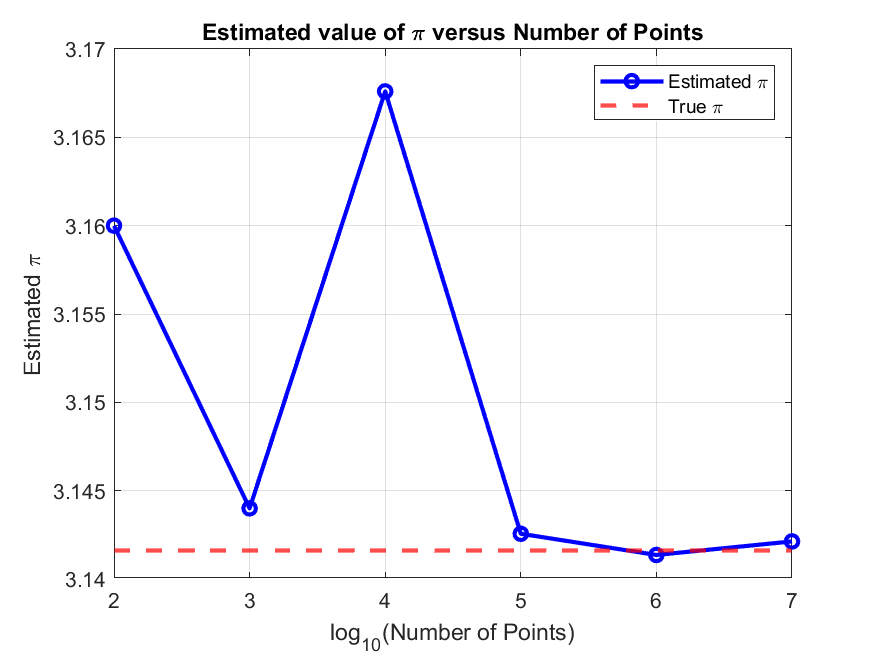
\includegraphics[width=0.8\textwidth]{Result_Files/pi_estimation_plot.png}
	\caption{Estimated value of $\pi$ versus number of points (log scale).}
	\label{fig:pi_estimation}
\end{figure}

As shown in Figure 1, the estimated value of $\pi$ approaches the true value as the number of points increases. The horizontal red dashed line represents the true value of $\pi$.

\begin{figure}[H]
	\centering
	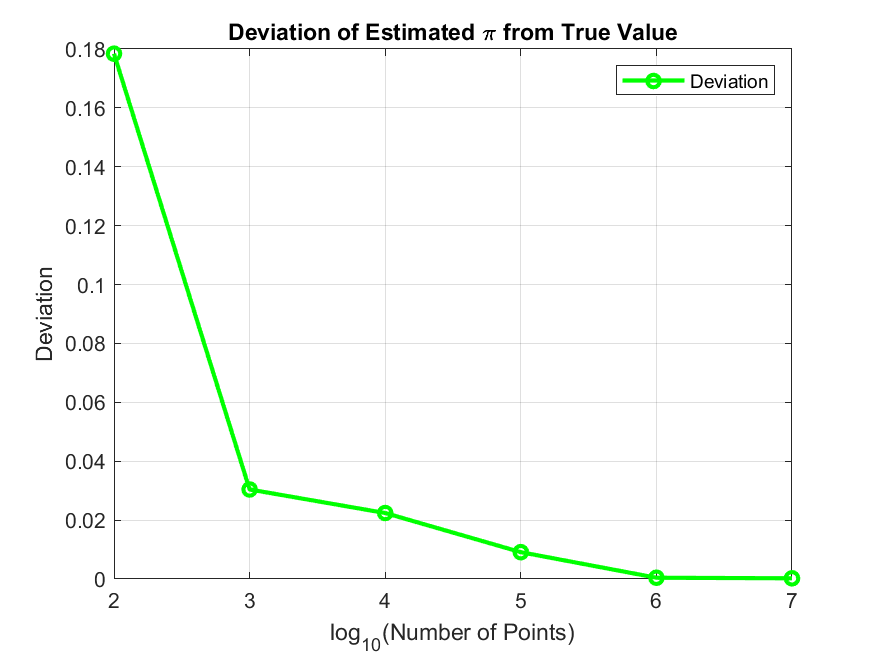
\includegraphics[width=0.8\textwidth]{Result_Files/pi_deviation_plot.png}
	\caption{Deviation of estimated $\pi$ from the true value.}
	\label{fig:pi_deviation}
\end{figure}

Figure 2 shows how the deviation from the true value of $\pi$ decreases as more points are sampled, indicating that the method converges.

\subsection{Execution Time}
\begin{figure}[H]
	\centering
	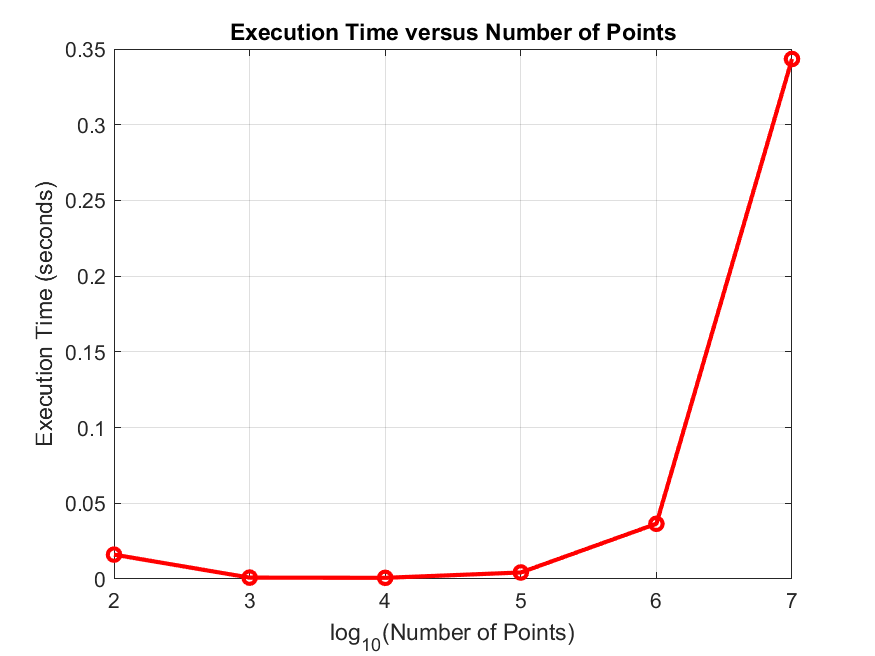
\includegraphics[width=0.8\textwidth]{Result_Files/execution_time_plot.png}
	\caption{Execution time versus number of points (log scale).}
	\label{fig:execution_time}
\end{figure}

Also in Figure 3, we can see that the execution time increases with the number of points. Larger datasets require more computational effort, which is reflected in the growing time complexity.

\subsection{Precision vs Computational Cost}
\begin{figure}[H]
	\centering
	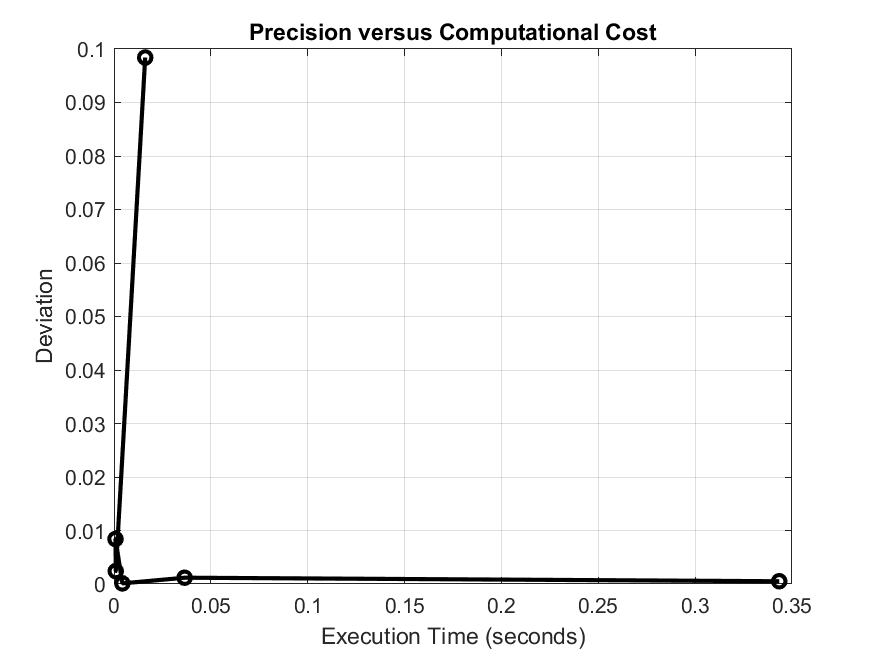
\includegraphics[width=0.8\textwidth]{Result_Files/precision_vs_cost_plot.png}
	\caption{Precision versus computational cost (execution time).}
	\label{fig:precision_cost}
\end{figure}

Figure 4 shows the trade-off between computational cost (execution time) and precision. As the number of points increases, precision improves but at a higher computational cost.

\section{Monte Carlo Estimation to a Specified Precision}
\subsection{Methodology}
In the second part of the experiment, the aim is to achieve a target precision (e.g., 0.001). The algorithm iteratively increases the number of random points until the deviation between successive estimates of $\pi$ falls below the specified precision threshold. The loop terminates when the target precision is met or when a maximum number of iterations is reached.

\subsection{Results}
The final estimate of $\pi$ for a precision target of $0.001$ was obtained after several iterations. A total of $N$ points were used, and the number of iterations was $X$.

\begin{figure}[H]
	\centering
	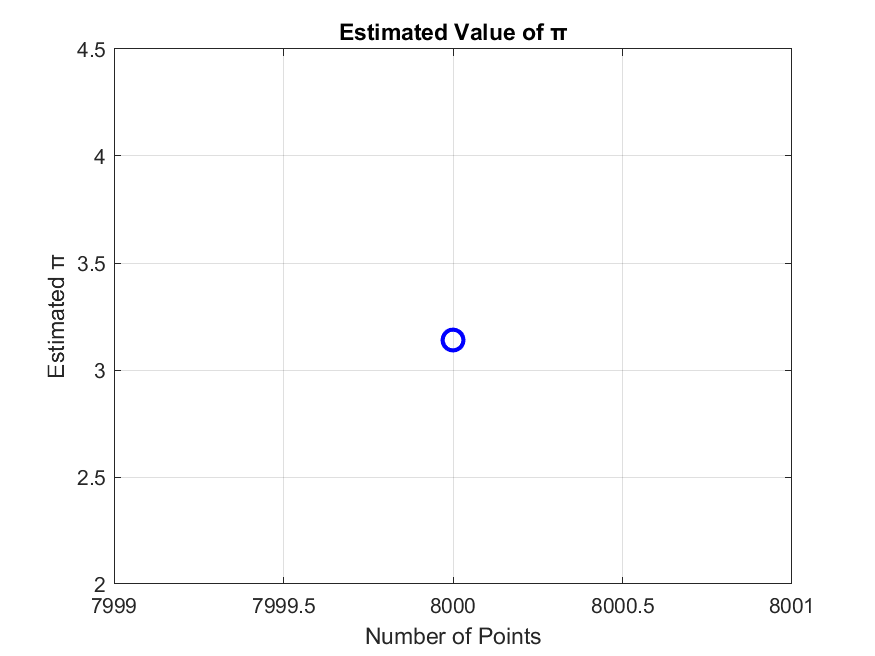
\includegraphics[width=0.8\textwidth]{Result_Files/pi_estimation_precision_plot.png}
	\caption{Estimated value of $\pi$ to a specified precision.}
	\label{fig:precision_estimation}
\end{figure}

\section{Monte Carlo Estimation with Simulation}
\subsection{Methodology}
In the third part, I created a function that estimates $\pi$ to a specified precision while generating a GIF that visualizes the points inside and outside the quarter circle. This process allows for real-time visualization of the convergence of the estimate.

\subsection{Results}
The output is a GIF file showing the iterative process of random point generation and the final estimated value of $\pi$.

\begin{figure}[H]
	\centering
	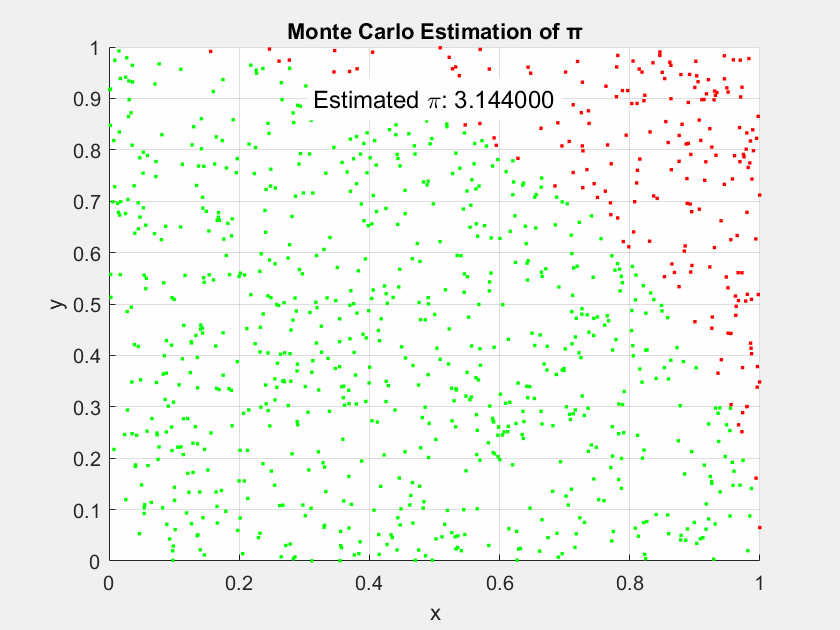
\includegraphics[width=0.8\textwidth]{Result_Files/monte_carlo_simulation.png}
	\caption{Visualization of Monte Carlo estimation of $\pi$ (Simulation on Github).}
	\label{fig:gif_visualization}
\end{figure}

\section{Conclusion}
The Monte Carlo method provides an intuitive and relatively simple approach to estimate $\pi$. However, achieving high precision requires a significant number of points, and thus greater computational cost. The trade-off between precision and execution time should be considered when selecting the number of points. The visualization through a simulation allows for real-time observation of the convergence of the estimate.

\begin{thebibliography}{1}

	\bibitem{chatgpt}
	OpenAI, ChatGPT Version 4 - \url{https://www.openai.com/chatgpt}. \textbf{\underline{This was used only for these purposes}}:
	\begin{enumerate}
		\item Assisted in converting the image to GIF format for the Section-3 of the assignment.
		\item Provided the idea to use a log scale for data points instead of a linear scale.
		\item Guidance on formatting and best coding practices.
	\end{enumerate}

	\bibitem{montecarlo}
	\url{https://en.wikipedia.org/wiki/Monte_Carlo_method}

	\bibitem{montecarlo}
	\url{https://www.mathworks.com/help/matlab/graphics-images.html}
\end{thebibliography}
\end{document}
